\section{Deployment and component placement}\label{sec:deployment}

Everything that matters runs on one laptop. So deployment is about how the
system is built from processes, not where they sit in the world. There are two
processes and two browser tabs. They talk only through the interfaces of
Section~\ref{sec:interfaces}. One optional call leaves the machine. When the language model is the
chosen detector, it runs on a shared server on the university network.

\begin{figure}[H]
\centering
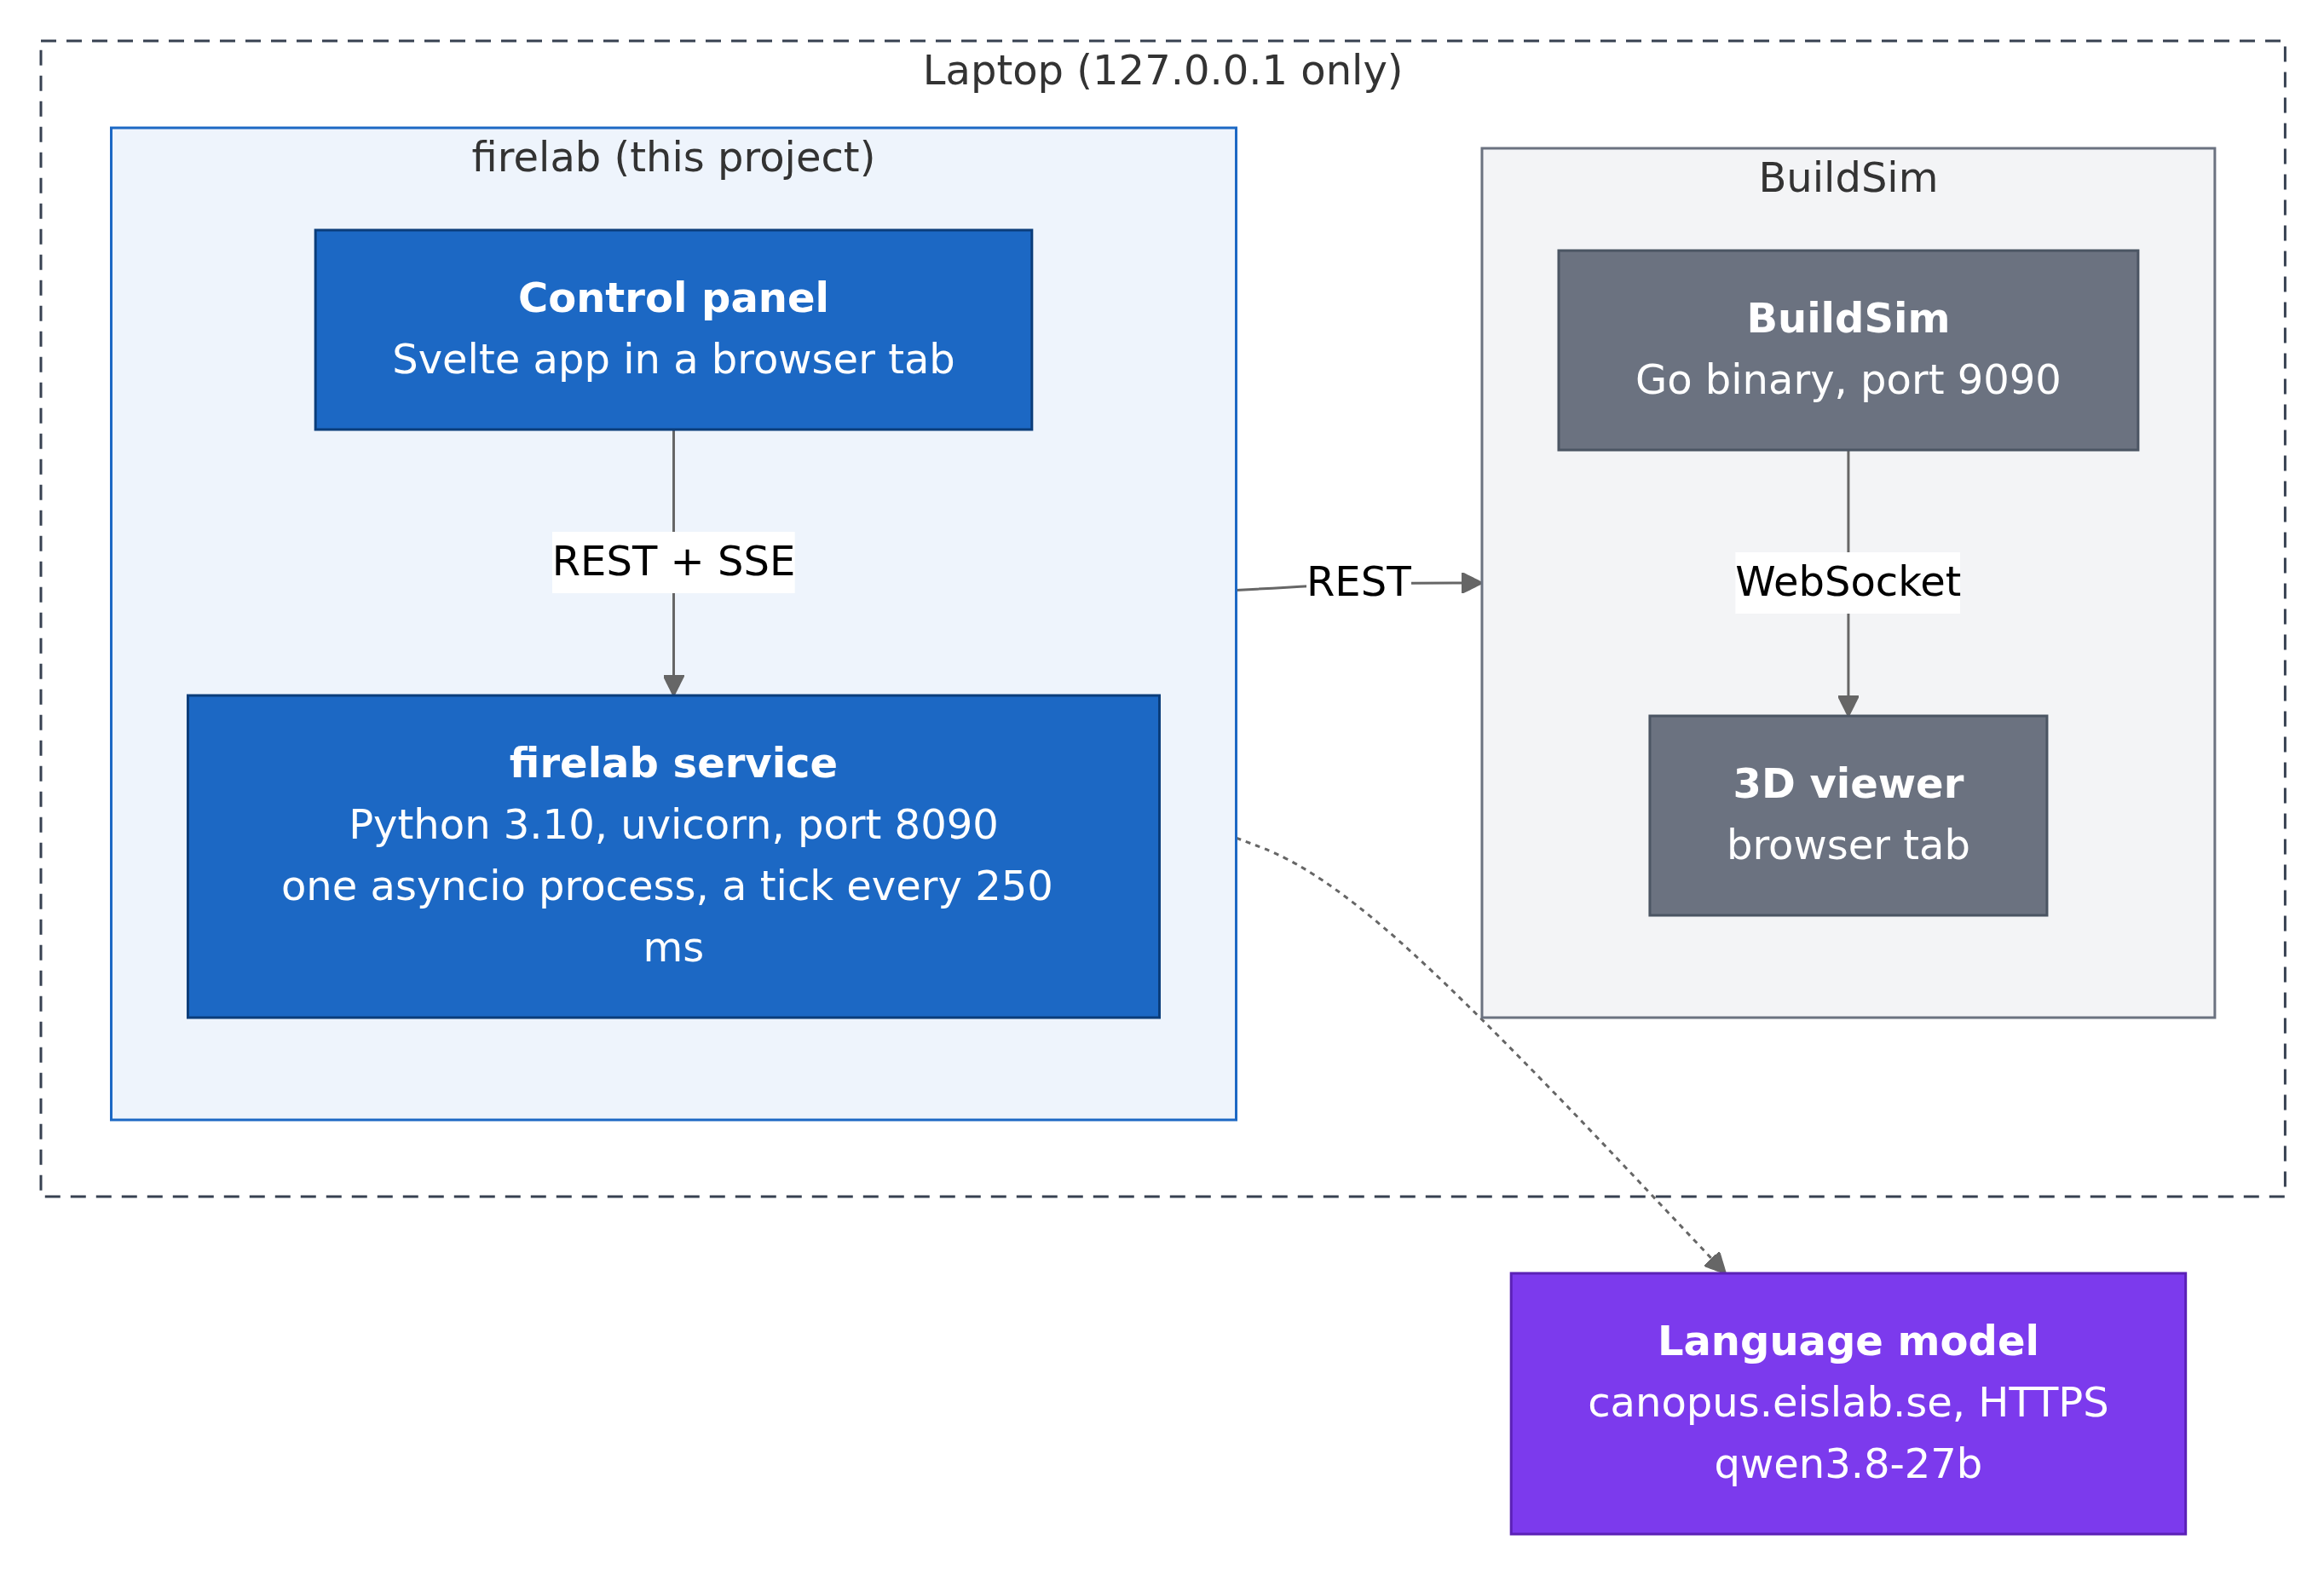
\includegraphics[width=0.95\linewidth]{images/deploy.png}
\caption{Deployment view: two processes, two tabs, loopback only. The purple box, reached by the dotted arrow, is the only part that leaves the laptop. The system keeps detecting without it.}
\label{fig:deploy}
\end{figure}

\textbf{Why this placement.} The control loop lives in the firelab process. It
runs from the physics, through the sensors, to the safety rules (interlocks) and
back. It touches nothing outside the machine except BuildSim over loopback. In a
real building, this process is the edge node. It must keep working when the
internet does not. It must also answer within the tick budget, which Section~\ref{sec:evaluation}
measures. The model endpoint puts that idea to the test. It is off the edge, it
is slow, and someone else runs it. So the adapter treats it as advice, not as
something the system depends on. The rule scores every room the model has not
answered for. The tick never waits for the call. If the endpoint disappears, the
journal says so and nothing else changes. A real building would need this design
for any cloud service on the detection path. That is why the box is dotted.
BuildSim stands in for the building's own controllers, and I left it alone.

\textbf{What is lost by merging the zones into one process}, since the course
asks: fault isolation and independent restart. If the physics crashes, the agent
dies with it. That is fine for a simulator on a laptop, but not for a building.
The safeguard I built in is the layering. It keeps the zones as easy to separate
as separate processes would. I also know where to split. The sensing zone already
produces readings per device, keyed by device ID. The actuation zone already takes
commands with a reason. Those are the two messages a broker would carry.

\textbf{Operational notes.} You start the service with \code{make run}. This
creates a virtual environment, builds the panel and serves it. Configuration is
live. Speed, thresholds, waiting times, sensor noise and population change on the
next tick through \code{PUT /api/config}. A reload re-reads the floors from
BuildSim without a restart. If BuildSim is down at startup, the service says so in
its journal and sits idle until a reload. If BuildSim goes away mid-run, the
service marks itself disconnected and stops writing. It keeps simulating.

\section{Test plan}\label{sec:testplan}

Two kinds of evidence back the requirements. The first is the unit suite: 162
tests and 98 subtests in 22 files. It runs in three seconds with nothing else
running. That works because the domain imports nothing that needs a network. The
model detector is tested against a fake endpoint and a fake clock. The second is
the experiments (E1 to E7). They drive the real engine tick by tick against the
loaded building, with publishing switched off. They use the same seed every time
and write their measurements to \code{experiments/results/}. E7, the model
comparison, is the only one that also needs the endpoint and a wall clock.
Section~\ref{sec:evaluation} reports them.

\begin{longtable}[]{@{}
  >{\raggedright\arraybackslash}p{(\columnwidth - 6\tabcolsep) * \real{0.12}}
  !{\colsep}>{\raggedright\arraybackslash}p{(\columnwidth - 6\tabcolsep) * \real{0.44}}
  !{\colsep}>{\raggedright\arraybackslash}p{(\columnwidth - 6\tabcolsep) * \real{0.16}}
  !{\colsep}>{\raggedright\arraybackslash}p{(\columnwidth - 6\tabcolsep) * \real{0.28}}@{}}
\toprule
\rowcolor{tablehead}
\textbf{ID} & \textbf{Test} & \textbf{Requirement} & \textbf{Evidence} \\
\midrule
\endhead
T-1 & \code{test\_agent}: the ladder climbs one step at a time and respects every waiting time. Only \textsc{confirmed} and \textsc{clearing} send commands & FR-01, FR-04 & unit, passes \\
\rowline
T-2 & \code{test\_detector}: P(fire), the estimated chance of fire in a room, equals the sum of its parts. A room with no sensors gives no opinion. Cooking scores below the confirm threshold & FR-03, FR-06 & unit, passes \\
\rowline
T-3 & \code{test\_interlocks}: water is refused below 35\,°C. Lock is always refused. Close is refused when the room is occupied or on a route & SR-01 to SR-03 & unit, passes \\
\rowline
T-4 & \code{test\_sensing}: lag, rounding (quantisation), clamping and each of the four faults behave as specified & NFR-02 & unit, passes \\
\rowline
T-5 & \code{test\_physics}, \code{test\_sources}: relaxation, the diffusion cap, sprinkler factors, the $t^2$ curve & Section~\ref{sec:physics} & unit, passes \\
\rowline
T-6 & \code{test\_evacuation}, \code{test\_walkways}, \code{test\_multifloor}: clear routes avoid danger, upper floors reach a ground-floor exit, and the drawn route starts at the fire & FR-05 & unit, passes \\
\rowline
T-7 & \code{test\_scoring}, \code{test\_history}: the catch, miss and false-alarm rules. The RSET milestones (RSET is the time from ignition until the last person is out). The recorder's columns and length & FR-07 & unit, passes \\
\rowline
T-8 & \code{test\_layering}: the direction of imports and the truth boundary & NFR-04 & unit, passes \\
\rowline
T-9 & \code{test\_publishing\_route}, \code{test\_publisher\_doors}: the route is sent only when it changes, and it names its storeys. Closed doors reach BuildSim & NFR-05 & unit, passes \\
\rowline
T-10 & \code{test\_reset}, \code{test\_presets}: a reset returns to a quiet building and forgets injected faults. Every preset is well formed & NFR-03 & unit, passes \\
\rowline
T-11 & \code{test\_llm\_detector}: the prompt carries readings only. A good reply becomes an answer, and a bad one is refused. The rule answers until the model has spoken, and again once the model's answer expires. A quiet room costs no question. Each room gets one question at a time, the most suspicious first. The speed limit follows measured answer times & FR-06, FR-08, NFR-06, NFR-07 & unit, passes \\
\rowline
T-12 & \code{test\_pacing}: the rule has no speed limit. A slow detector caps the speed dial once and says so. Switching back lifts the cap & NFR-07 & unit, passes \\
\rowline
E1 & Each of the six presets in A3505 for 20 simulated minutes: state times, score, response, peak truth & FR-01 to FR-04, SR-01 & Table~\ref{tab:presets}, Figure~\ref{fig:office} \\
\rowline
E2 & The office fire with the agent's commands dropped (supervised mode), then with the sprinkler alone & Section~\ref{sec:physics} loop & Table~\ref{tab:contain} \\
\rowline
E3 & Office fire and kitchen cooking at sensor noise 0, 1, 2, 3$\times$ & FR-03, NFR-03 & Table~\ref{tab:noise} \\
\rowline
E4 & Office fire with the smoke detector stuck, dropping out, drifting, or dead & NFR-02 & Table~\ref{tab:faults} \\
\rowline
E5 & Sensors in 10 to 956 rooms; wall time of one tick at 1$\times$ and 40$\times$ & NFR-01 & Figure~\ref{fig:scaling} \\
\rowline
E6 & Every experiment rerun from the same seed & NFR-03 & identical latencies to the second \\
\rowline
E7 & The six presets, cooking at 2 and 3$\times$ noise, and the fire with a stuck smoke detector, scored by the language model at the speed it can keep up with & FR-08, NFR-06, NFR-07 & Table~\ref{tab:detectors}, Figure~\ref{fig:detectors} \\
\bottomrule
\end{longtable}

\section{Evaluation and experiments}\label{sec:evaluation}

This section reports what I measured. The experiment harness in
\code{experiments/run\_experiments.py} measured every number below. It ran on the
loaded A-building, with the fire in office A3505 on the top floor. There were 130
people, placed by the default seed, and the thresholds were the defaults. The fire
room and its neighbours had all three sensor types, as the presets do.

\textbf{Detection and response (E1).}

\begin{table}[H]
\centering
\footnotesize
\resizebox{\linewidth}{!}{\begin{tabular}{@{}l!{\colsep}c!{\colsep}c!{\colsep}c!{\colsep}c!{\colsep}c!{\colsep}c!{\colsep}c@{}}
\toprule
\rowcolor{tablehead}
\textbf{Preset} & \textbf{Investigating} & \textbf{Confirmed} & \textbf{Max P(fire)} & \textbf{False alarms} & \textbf{Sprinkler} & \textbf{RSET} & \textbf{Outcome} \\
\midrule
Office fire (flaming, fast) & 51\,s & 106\,s & 0.994 & 0 & on at 106\,s & 217\,s & caught ✓ \\
\rowline
Overnight smoulder & 136\,s & 201\,s & 0.991 & 0 & refused 201\,s, on 219\,s & 312\,s & caught ✓ \\
\rowline
Kitchen cooking & 326\,s & never & 0.688 & 0 & & & correctly ignored ✓ \\
\rowline
Dust storm & never & never & 0.129 & 0 & & & correctly ignored ✓ \\
\rowline
Fire, dead smoke detector & 61\,s & never (room); 156\,s (neighbour) & 0.748 & 0 & on next door & 267\,s & caught by the neighbour, see below \\
\rowline
Drifting sensor, no fire & never & never & 0.057 & 0 & & & correctly ignored ✓ \\
\bottomrule
\end{tabular}}
\caption{One run of each preset. Times are in seconds since ignition. RSET runs from ignition until the last of 130 people is out. In every caught case, the building was empty 111\,s after the alarm.}
\label{tab:presets}
\end{table}

Both fires were confirmed well within the 180\,s and 300\,s limits of FR-01 and
FR-02. None of the three no-fire presets (cooking, dust and the drifting sensor)
raised an alarm (FR-03). Figure~\ref{fig:office} shows the office fire as the
system saw it. The truth and the reading agree until the heat detector maxes out
at 250\,°C. The probability climbs through the three thresholds. The waiting
times show as the flat time between crossing a level and changing state. After the
sprinkler starts at 106\,s, the true smoke bends down. The temperature keeps
rising in the now sealed room. The smoulder shows the safety rules at work. It was
confirmed on CO with the room at 34\,°C. Its sprinkler request was refused for
lack of heat, and the journal logged this. The request was granted 18\,s later,
when the room passed 35\,°C. The design worked as intended, but the number
deserves a second look. A limit of 35\,°C is a low bar for ``heat
corroboration'' (backing from a heat reading). A warm summer office would pass it.

\begin{figure}[H]
\centering
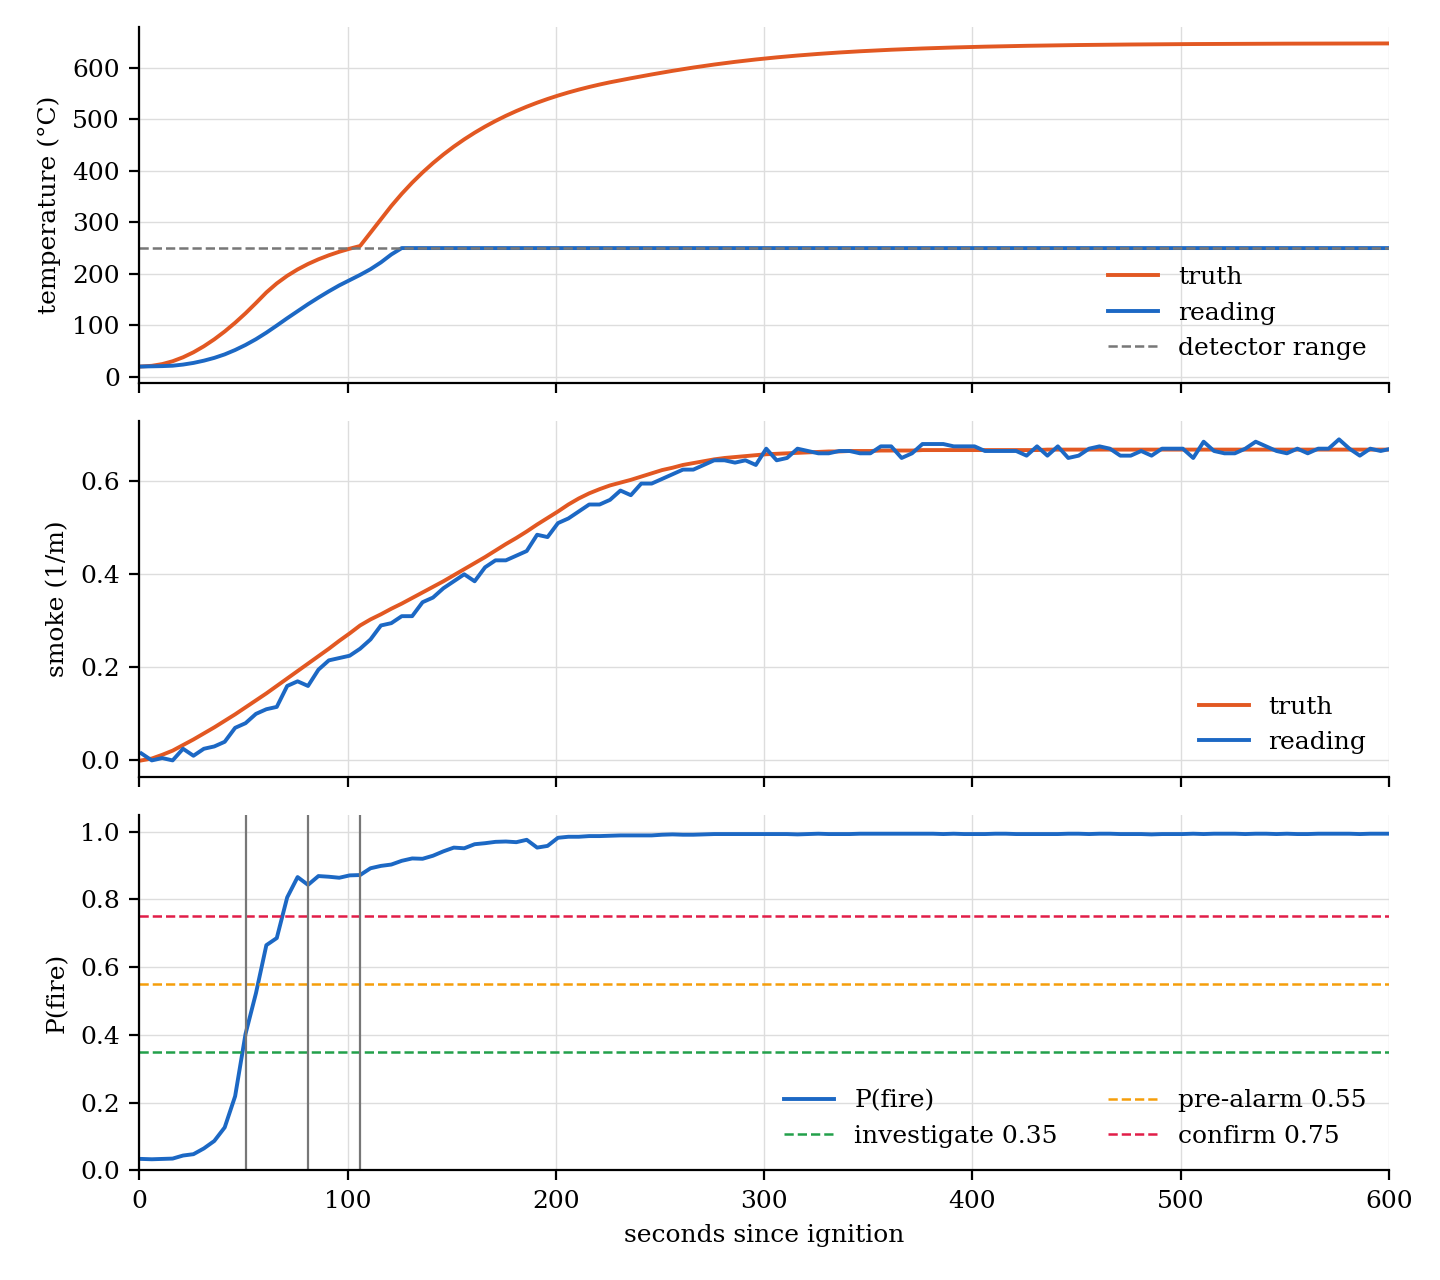
\includegraphics[width=0.92\linewidth]{images/chart_office_fire.png}
\caption{The first ten minutes of the office fire in A3505, as the system saw it (E1). Top: the heat detector maxes out at 250\,°C while the room reaches 648\,°C. Middle: smoke. The reading follows the truth with a 12\,s lag. Bottom: P(fire) passing the three thresholds. The vertical lines are the state changes at 51, 81 and 106\,s. The flat stretches before them are the waiting times.}
\label{fig:office}
\end{figure}

\textbf{The blind spot.} The preset with a dead smoke detector is the one result
that did not go to plan. Heat and CO alone pushed the fire room to a probability of
0.748. The coverage factor held it there. This factor caps a room with two working
sensor types at 85\,\% of its logistic score. The confirm threshold is 0.75. So
the room sat in \textsc{pre-alarm} for the whole run, three thousandths short. The
building was still evacuated at 156\,s. Smoke crossed into A3500A next door, and
its three working detectors confirmed. The fire room also fed A3500A's
neighbour-agreement term. I took two lessons from this. First, the neighbour
cross-check is not decoration: it is what caught this fire. Second, the coverage
penalty is tuned slightly too hard. Two changes would have confirmed the room
itself. One is lowering the penalty by raising its floor from 0.55 to 0.60. The
other is letting a neighbour's confirmation lift the room. This is the first
change I would make.

\textbf{Closing the loop, and what containment actually does (E2).}

\begin{table}[H]
\centering
\footnotesize
\resizebox{\linewidth}{!}{\begin{tabular}{@{}l!{\colsep}c!{\colsep}c!{\colsep}c!{\colsep}c!{\colsep}c@{}}
\toprule
\rowcolor{tablehead}
\textbf{Response} & \textbf{Rooms lost} & \textbf{Neighbour peak smoke} & \textbf{Neighbour peak temp} & \textbf{Fire room peak temp} & \textbf{RSET} \\
\midrule
None (supervised, nobody presses) & 5 & 0.382\,1/m & 149\,°C & 309\,°C & no evacuation \\
\rowline
Autonomous & 4 & 0.171\,1/m & 152\,°C & 648\,°C & 217\,s \\
\rowline
Sprinkler only, door held open & 5 & 0.171\,1/m & 152\,°C & 648\,°C & 217\,s \\
\bottomrule
\end{tabular}}
\caption{The same office fire three times. ``Rooms lost'' are rooms that became untenable at any point in 20 minutes. Untenable means unsafe for people to stay in, judged by the limits in the ISO 13571 standard.}
\label{tab:contain}
\end{table}

The response halves the smoke that reaches the neighbours and saves one room. It
also makes the fire room hotter. That surprised me until the journal explained it.
With the door open, the fire room dumps heat into five neighbours every step. With
the doors closed, it keeps the heat. The sprinkler's 25\,\% factor does not make
up for that. In this model, water reduces the heat the fire releases. It does
nothing to cool the room directly. The third row tells me more. Holding the fire
room's own door open made no difference at all. At 231\,s the neighbour A3500A
confirmed on the smoke that had crossed into it. It then closed \emph{its} doors,
and one of them is the same doorway. So in this building, containment depends on
every room around the fire, not on the fire room alone. Without any response,
nobody is told to leave and no RSET is recorded. That is the simplest argument for
making the evacuate command automatic.

\textbf{Noise (E3) and lying sensors (E4).}

\begin{table}[H]
\centering
\footnotesize
\begin{minipage}[t]{0.47\linewidth}
\centering
\begin{tabular}{@{}l!{\colsep}c!{\colsep}c!{\colsep}c!{\colsep}c@{}}
\toprule
\rowcolor{tablehead}
\textbf{Noise} & \multicolumn{2}{c}{\textbf{Office fire}} & \multicolumn{2}{c}{\textbf{Kitchen cooking}} \\
\rowcolor{tablehead}
 & confirmed & max P & alarms & max P \\
\midrule
0$\times$ & 106\,s & 0.994 & 0 & 0.447 \\
\rowline
1$\times$ & 106\,s & 0.994 & 0 & 0.688 \\
\rowline
2$\times$ & 106\,s & 0.995 & 0 & 0.749 \\
\rowline
3$\times$ & 106\,s & 0.996 & 0 & 0.741 \\
\bottomrule
\end{tabular}
\caption{Sensor noise sweep (E3).}
\label{tab:noise}
\end{minipage}\hfill
\begin{minipage}[t]{0.47\linewidth}
\centering
\begin{tabular}{@{}l!{\colsep}c!{\colsep}c@{}}
\toprule
\rowcolor{tablehead}
\textbf{Smoke detector} & \textbf{Confirmed} & \textbf{Max P} \\
\midrule
healthy & 106\,s & 0.994 \\
\rowline
dropout (40\,\% lost) & 101\,s & 0.995 \\
\rowline
drift & 106\,s & 0.995 \\
\rowline
stuck & 156\,s & 0.880 \\
\rowline
dead & never (neighbour 156\,s) & 0.748 \\
\bottomrule
\end{tabular}
\caption{Faults on the fire room's smoke detector during the office fire (E4).}
\label{tab:faults}
\end{minipage}
\end{table}

Detection time did not move by a second across the noise sweep, and cooking never
raised an alarm. That is the waiting times doing their job. The number to worry
about is the cooking peak at 2$\times$ noise: 0.749 against a confirm threshold of
0.75. It did not confirm. To confirm, it would first have to hold 0.55 for 20\,s
and then sit 25\,s in pre-alarm, and it never did. But the margin on the
probability itself is only one noise sample wide. The CO term is what keeps
cooking down. So, to be accurate, this detector tells cooking from fire by CO and
time, not by any single reading. On faults, a detector that dropped readings
caught the fire slightly faster. The readings it did send happened to land on
rising edges. A stuck detector cost 50\,s, because the rate term went flat. Drift
did nothing in twenty minutes. A dead detector is the blind spot above.

\textbf{Scaling and the breaking point (E5).} The tick loop wakes every 250\,ms
of real time. It must finish before it wakes again. At 1$\times$ speed, one tick is
one physics step over the whole building plus one intelligence pass over the
monitored rooms. At 40$\times$ it is forty physics steps and one pass.

\begin{figure}[H]
\centering
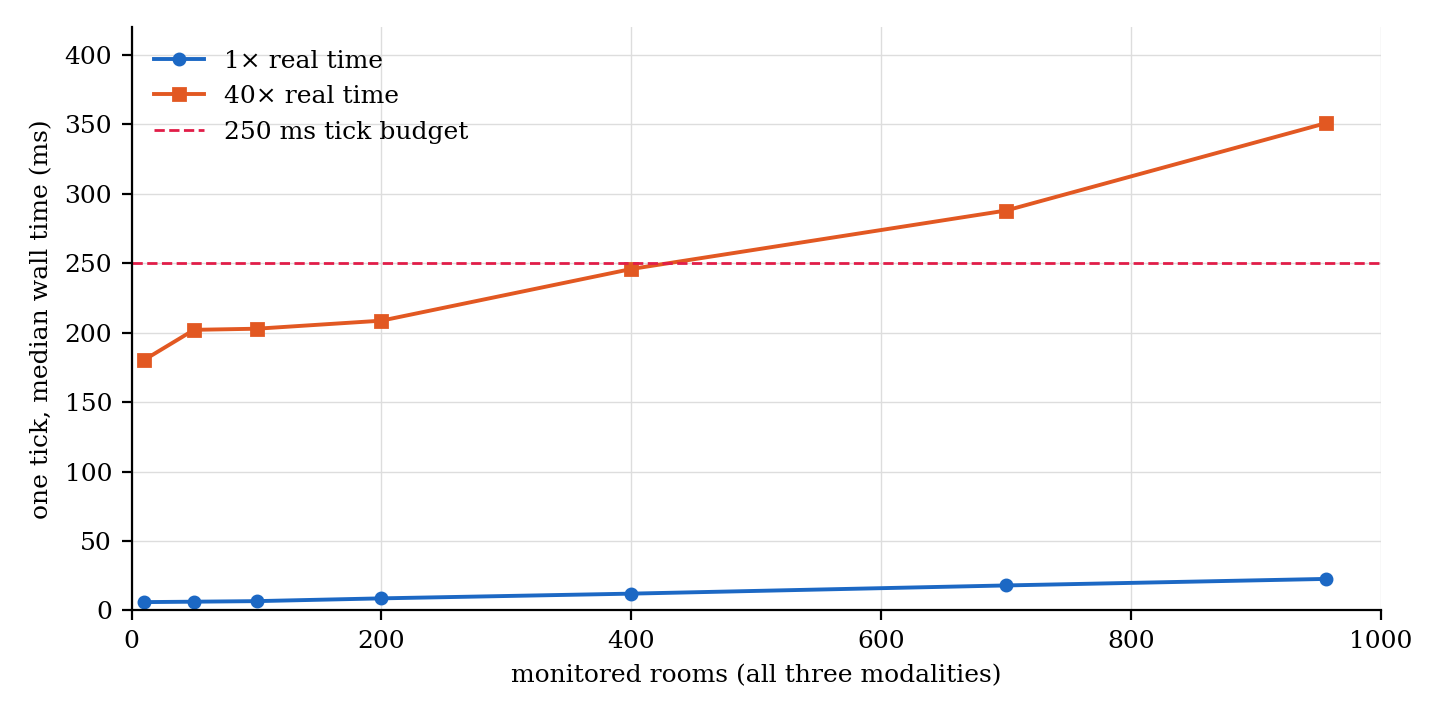
\includegraphics[width=0.86\linewidth]{images/chart_scaling.png}
\caption{Real (wall-clock) time of one engine tick against the number of monitored rooms (E5), on the laptop the demo runs on. The building has 956 rooms and 1005 doorways.}
\label{fig:scaling}
\end{figure}

At real time the whole building fits with room to spare: 23\,ms per tick with all
956 rooms monitored and 2868 devices sampling. At 40$\times$ the tick goes over
budget at about 450 monitored rooms. The shape of the curve shows where the cost
is. With only 10 rooms monitored, a 40$\times$ tick already takes 180\,ms. So the
forty physics steps over the full graph are the fixed cost, about 4.5\,ms a step.
The intelligence adds about 0.18\,ms per monitored room on top. The physics cost
does not grow with the number of sensors. So for a bigger building or a faster
clock, the fix is a sparser diffusion step, not a faster detector. When the tick
goes over budget, nothing breaks. The loop just runs slower than the speed dial
claims. The tick also caps itself at sixty physics steps, so a stall cannot
snowball.

\textbf{The language model as the detector (E7).} I ran the same scenarios again
with the language model (\code{qwen3.8-27b} on the lab's server) deciding P(fire)
instead of the rule. The script is \code{experiments/compare\_detectors.py}. The
model is asked about one room at a time, and each answer is trusted for 60
simulated seconds. When the model has no recent answer, the rule fills in. So the
numbers below are for the model and the rule working together, not the model on
its own. These runs are slow because they wait for real answers: the nine of them
took 98 minutes.

\begin{table}[H]
\centering
\footnotesize
\resizebox{\linewidth}{!}{\begin{tabular}{@{}l!{\colsep}c!{\colsep}c!{\colsep}c!{\colsep}c!{\colsep}c!{\colsep}c!{\colsep}c!{\colsep}c@{}}
\toprule
\rowcolor{tablehead}
\textbf{Scenario} & \textbf{Rule: alarm} & \textbf{Model: alarm} & \textbf{Model max P} & \textbf{Model share} & \textbf{Answered / failed / asked} & \textbf{Median answer} & \textbf{Clock} \\
\midrule
Office fire & 106\,s & 136\,s & 0.99 & 57\,\% & 32 / 2 / 35 & 7.3\,s & 2.5$\times$ \\
\rowline
Overnight smoulder & 201\,s & 201\,s & 0.97 & 32\,\% & 16 / 5 / 22 & 14.8\,s & 2.3$\times$ \\
\rowline
Kitchen cooking, 1$\times$ noise & none & none & 0.22 & 39\,\% & 33 / 1 / 36 & 14.5\,s & 2.0$\times$ \\
\rowline
Kitchen cooking, 2$\times$ noise & none & none & 0.72 & 38\,\% & 33 / 2 / 36 & 15.1\,s & 2.0$\times$ \\
\rowline
Kitchen cooking, 3$\times$ noise & none & none & 0.76 & 43\,\% & 35 / 1 / 37 & 17.3\,s & 1.8$\times$ \\
\rowline
Dust storm & none & none & 0.07 & 92\,\% & 36 / 0 / 36 & 7.2\,s & 3.0$\times$ \\
\rowline
Fire, dead smoke detector & 156\,s (neighbour) & 156\,s (neighbour); room 798\,s & 0.90 & 18\,\% & 22 / 3 / 26 & 21.5\,s & 2.1$\times$ \\
\rowline
Drifting sensor, no fire & none & none & 0.08 & 86\,\% & 43 / 0 / 45 & 7.9\,s & 3.0$\times$ \\
\rowline
Office fire, stuck smoke detector & 156\,s & 156\,s & 0.93 & 57\,\% & 37 / 4 / 42 & 20.0\,s & 1.4$\times$ \\
\bottomrule
\end{tabular}}
\caption{The rule compared with the language model (E7). Alarm: when the first room in the building was confirmed, in seconds after the fire started. Model share: how much of the time the model, not the rule, was scoring the fire room. Clock: how fast the simulation could run so the model's answers were still fresh when they arrived.}
\label{tab:detectors}
\end{table}

\begin{figure}[H]
\centering
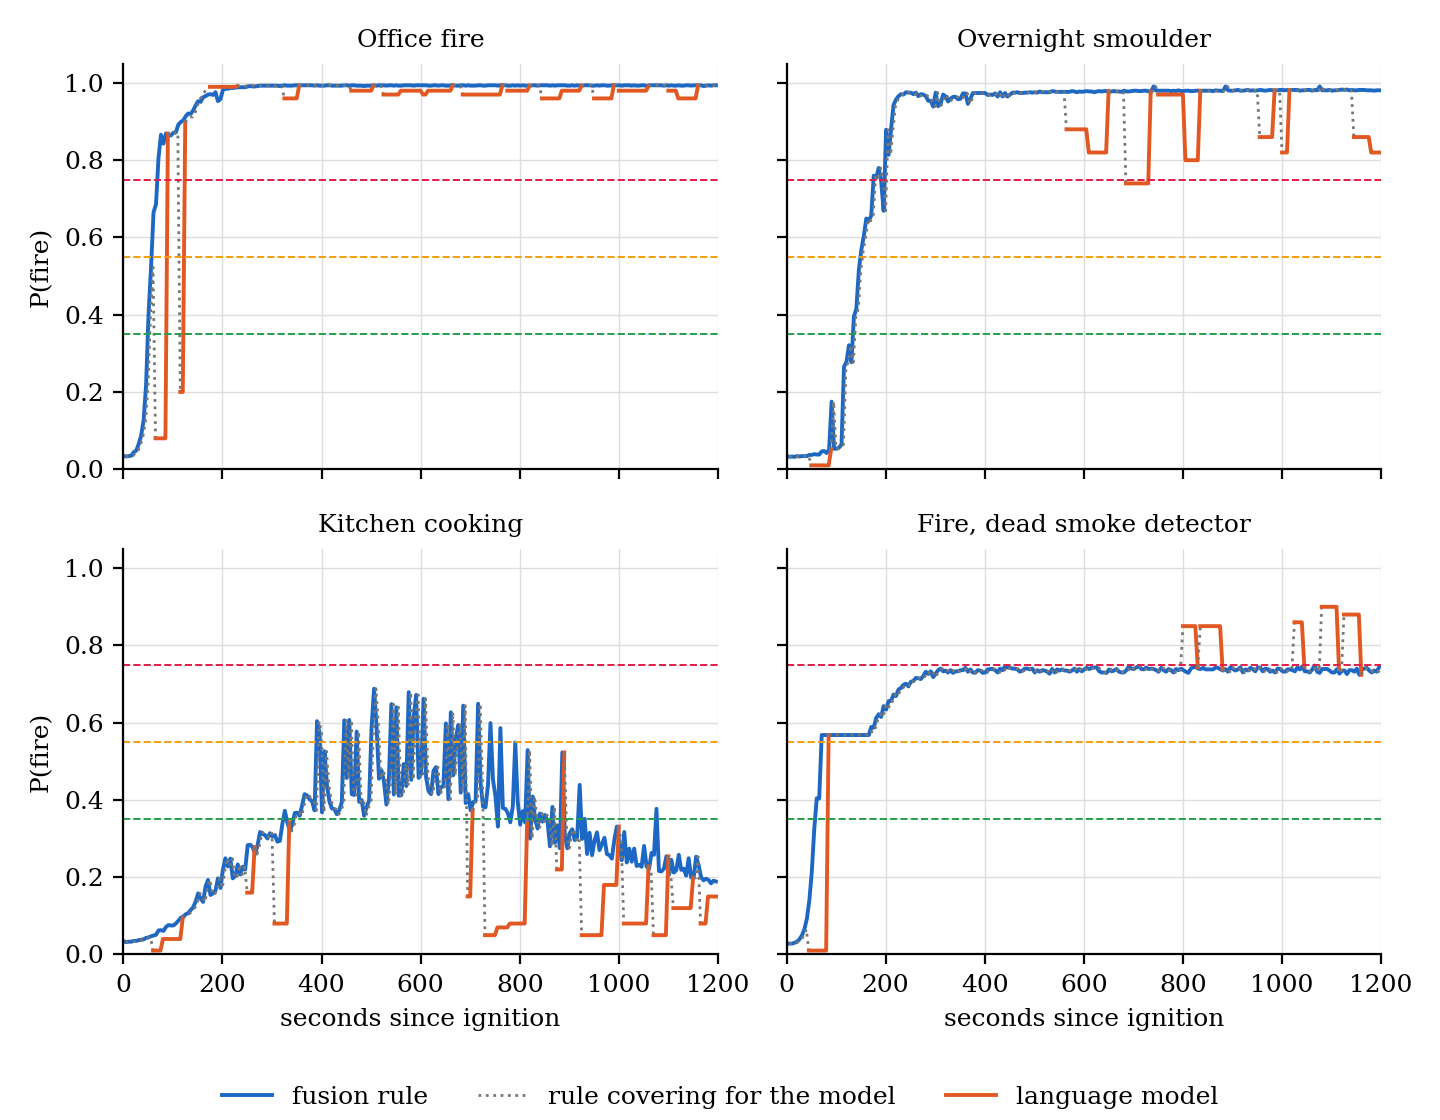
\includegraphics[width=0.92\linewidth]{images/chart_detectors.png}
\caption{P(fire) in the fire room with each detector (E7). Blue: the rule on its own. Orange: the model's answers. Grey dots: the rule filling in while the model had no recent answer. The dashed lines are the three alarm levels.}
\label{fig:detectors}
\end{figure}

In all nine runs the end result was the same as with the rule: every fire was
caught and nothing else set off an alarm. The differences are in how fast, and in
what it cost.

In the office fire, the model's first answers were low. Twice, at 64\,s and
116\,s, they sent the fire room back to \textsc{normal}, and the waiting time
started over. The alarm came 30\,s later than with the rule, and it came from the
room next door (A3500A). The fire room itself was confirmed at 170\,s.

With the dead smoke detector, the model did something the rule could not. It gave
the fire room 0.85 to 0.90, while the rule got stuck at 0.748, so the model
confirmed the room itself. But its answers about that room came so slowly that
this only happened at 798\,s. By then the room next door had already raised the
alarm, at 156\,s, in both runs.

For cooking, the model was calmer than the rule at normal noise (0.22 against
0.688). At three times the noise it was not: it reached 0.76, just over the
confirm level. The waiting times stopped it from raising an alarm, just as they
did for the rule.

The real cost is speed. A typical answer took 7 to 21\,s, and the slowest took
85\,s. 18 of 315 questions failed. The simulation could only run 1.4 to 3 times
faster than real time, while the rule manages 40 times. In the quiet runs the
model was scoring the fire room 86 to 92\,\% of the time, but in the fires only 18
to 57\,\%. So in the runs that mattered most, the rule did a lot of the work. The
results also change from run to run, even with the same seed, because what the
model is asked depends on how long its last answer took.

What the model gave me was a second opinion where the rule was too strict, and a
reason in the journal that a person can read. What it could not do was make
things worse than a delay. The waiting times, the safety rules and the rule
filling in all sit between the model's number and anything that happens in the
building.

\textbf{Headline results.}

\begin{table}[H]
\centering
\footnotesize
\resizebox{\linewidth}{!}{\begin{tabular}{@{}l!{\colsep}l!{\colsep}l!{\colsep}l@{}}
\toprule
\rowcolor{tablehead}
\textbf{Metric} & \textbf{Measured} & \textbf{Requirement} & \\
\midrule
Flaming fire confirmed & 106\,s & $\le 180$\,s (FR-01) & ✓ \\
\rowline
Smouldering fire confirmed & 201\,s & $\le 300$\,s (FR-02) & ✓ \\
\rowline
False alarms, 3 no-fire presets $\times$ 4 noise levels & 0 & 0 (FR-03) & ✓ \\
\rowline
Commands on confirmation & sprinkler, door, evacuate, same tick, with reasons & (FR-04) & ✓ \\
\rowline
Sprinkler refused without heat & yes, released 18\,s later & (SR-01) & ✓ \\
\rowline
Fire caught with a stuck, dropping or drifting smoke detector & yes, worst 156\,s & (NFR-02) & ✓ \\
\rowline
Fire room confirmed with a dead smoke detector & no; caught next door at 156\,s & (NFR-02) & partial \\
\rowline
Tick at 1$\times$, full building & 23\,ms & $\le 250$\,ms (NFR-01) & ✓ \\
\rowline
Breaking point at 40$\times$ & about 450 monitored rooms & measured (NFR-01) & ✓ \\
\rowline
Building of 130 cleared after the alarm & 111\,s & reported (FR-07) & ✓ \\
\rowline
Same seed, same run & identical to the second, every rerun & (NFR-03) & ✓ \\
\rowline
Language model as detector, 9 scenarios & all 4 fires caught, 0 false alarms & (FR-08) & ✓ \\
\rowline
Model answers never used when out of date & typical answer 7--21\,s; simulation held to 1.4--3$\times$ & (NFR-07) & ✓ \\
\bottomrule
\end{tabular}}
\end{table}

\section{Dashboard}\label{sec:dashboard}

The dashboard is two browser tabs. They are meant to be read together, and each
has its own job. The BuildSim viewer shows the building. It has heat maps of the
true temperature, smoke and CO on the floors. It shows flames and smoke in the
burning room, the sprinkler running, and every one of the 130 people walking.
Alarming rooms are outlined in red, orange or yellow by state. The one escape
route is a red line from the fire room, down the stairs, to a ground-floor exit.
The control panel shows the system: what it is told, what it believes, and what
it did about it.

\begin{figure}[H]
\centering
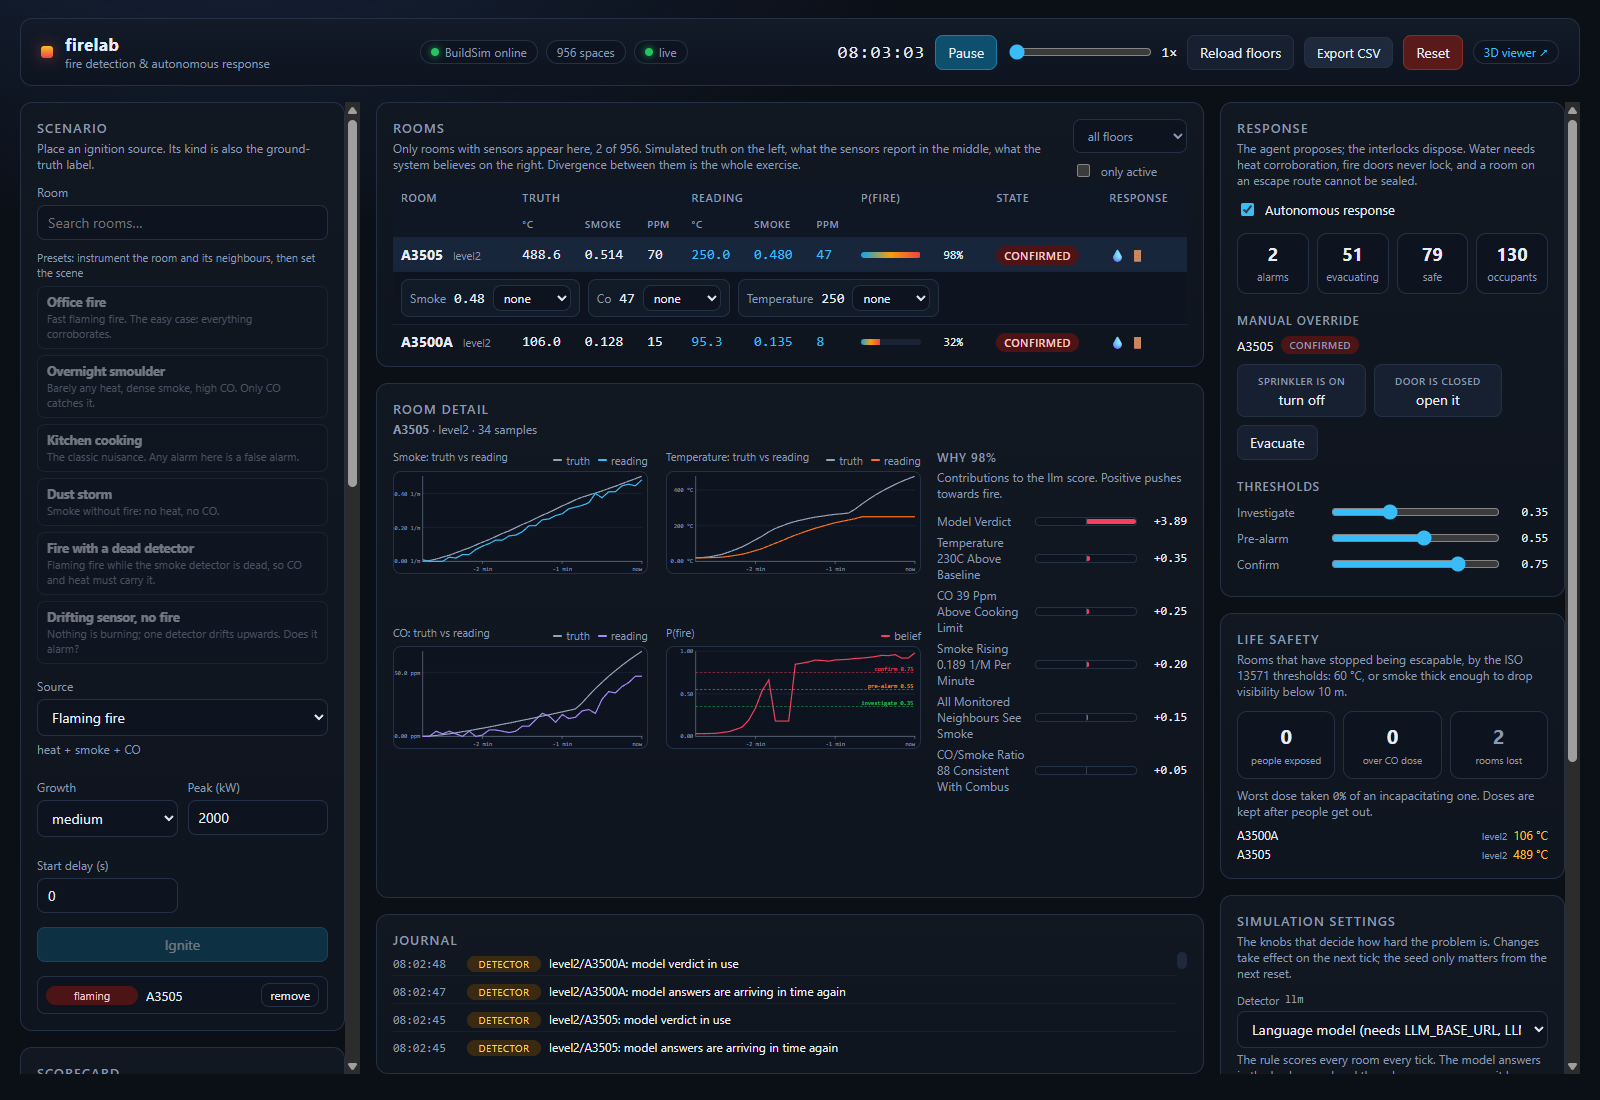
\includegraphics[width=\linewidth]{images/dashboard.png}
\caption{The control panel during the office fire, with the language model as the detector. Rooms table: truth on the left, readings in the middle, P(fire) and state on the right. Room detail: truth against reading for each sensor type, and the ``Why'' bars. Here the bars show the model's own evidence, with its answer as the top bar. Journal: the model's hand-overs. Bottom right: the detector selector.}
\label{fig:dashboard}
\end{figure}

\begin{figure}[H]
\centering
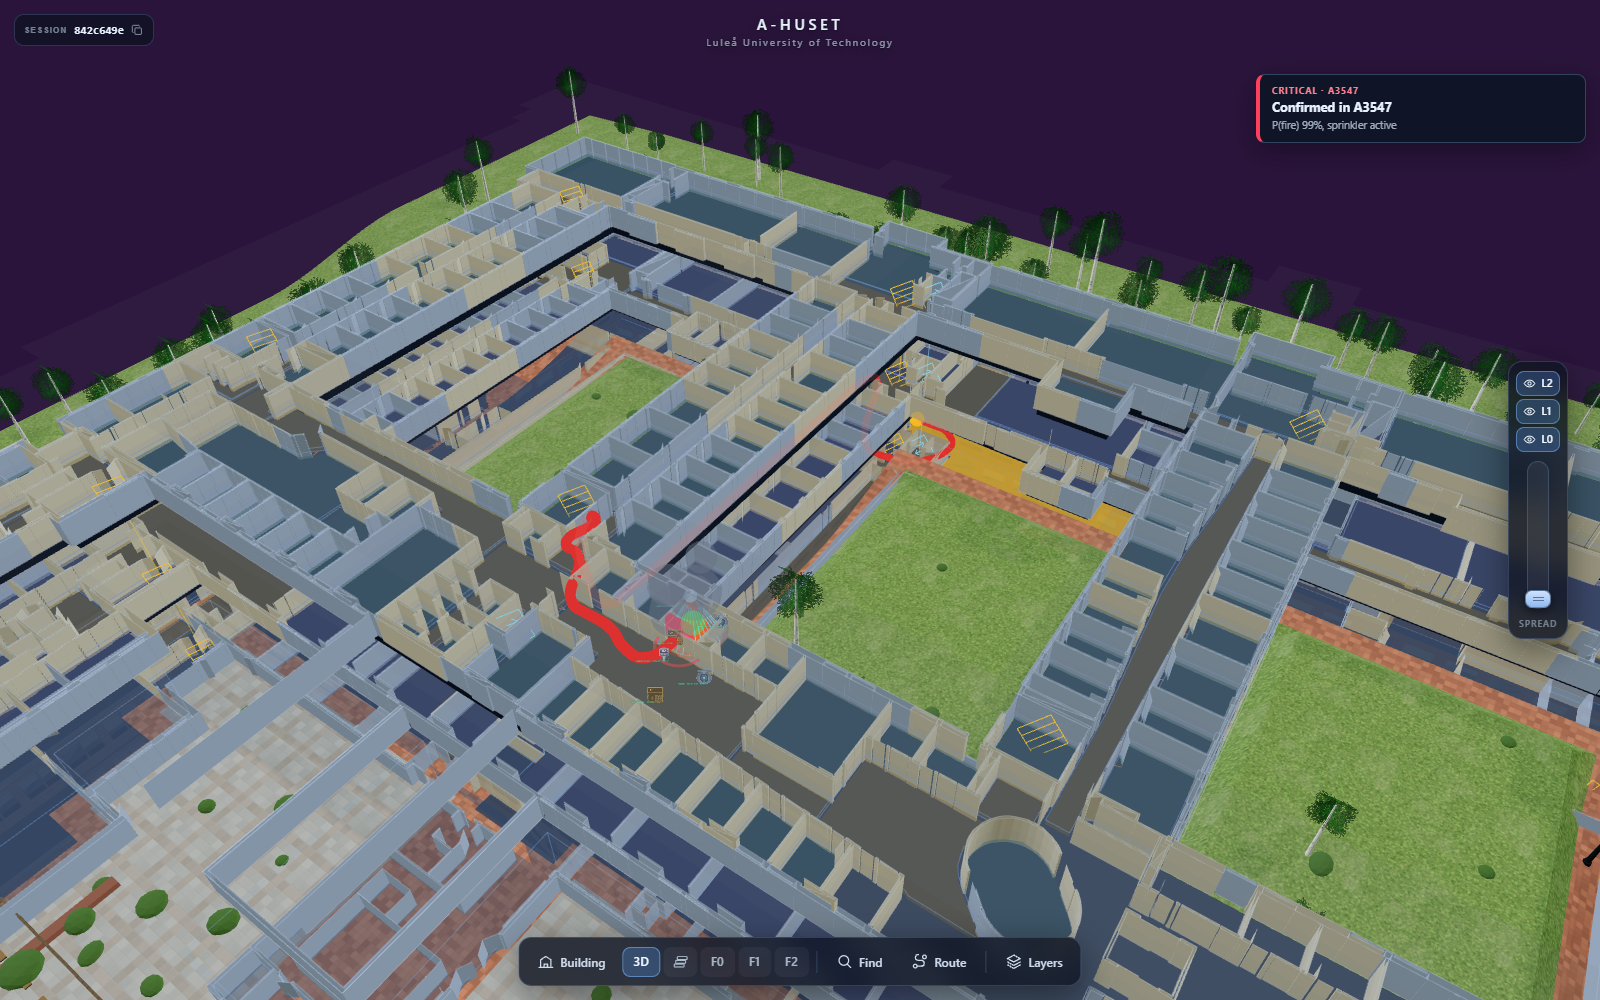
\includegraphics[width=0.49\linewidth]{images/viewer_route.png}\hfill
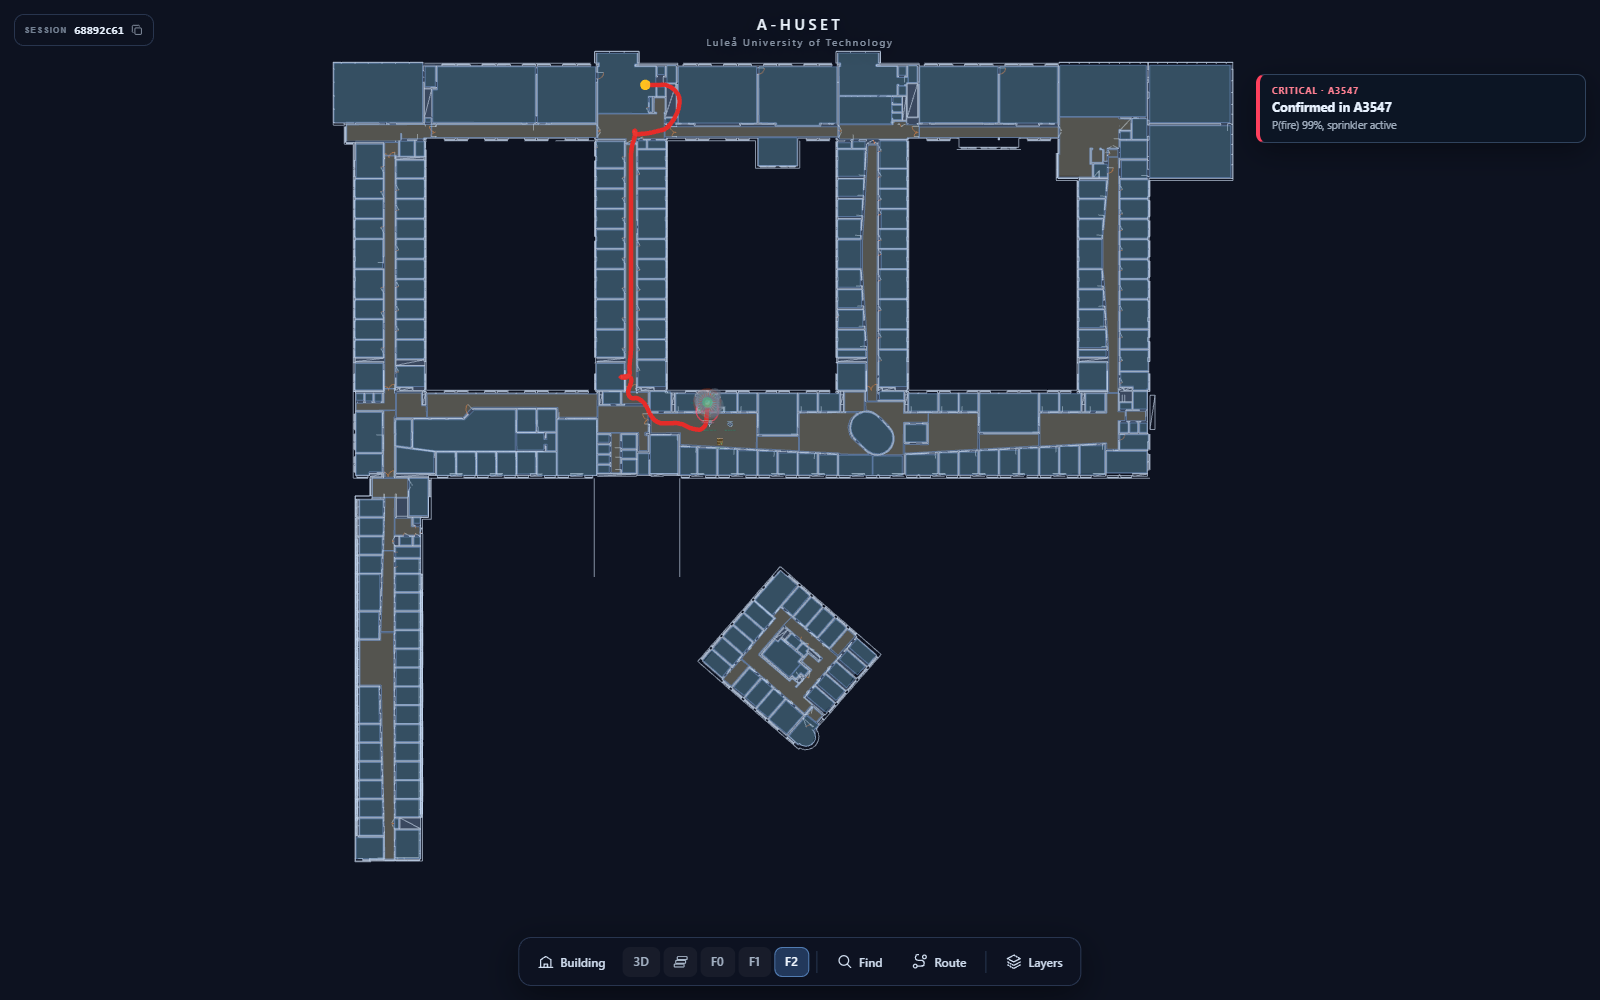
\includegraphics[width=0.49\linewidth]{images/viewer_plan.png}
\caption{The BuildSim viewer with firelab's overlays. Left: the 3D view, with the fire in the top-floor office and the escape route going down the stairwell. Right: the same route on the floor-2 plan, from the burning room to the exit.}
\label{fig:viewer}
\end{figure}

The most useful part of the panel is the least visual. The Rooms table puts the
true value of each sensor type next to what its sensor reported. The room detail
draws both on one chart. A maxed-out heat detector, a stuck smoke detector or a
drifting one shows up as a gap between two lines. The operator of a real building
never gets to see this, and it is what this project is about. Next to it, the
``Why'' bars split the probability into its parts. So 99\,\% is not a claim but a
sum. With the model installed, the same bars show what the model said it weighed,
with its answer as the top bar. The heading names which detector is speaking. The
P(fire) trace in Figure~\ref{fig:dashboard} shows the model's first answer
pulling the room back to normal before its second answer lifted it. A number on
its own would hide that. The journal below records every state change and every
command with its reason. It also records every refusal with the safety rule's
reason, and every hand-over between the model and the rule. The scorecard grades
the run as it happens: catches, misses, false alarms, the alarm delay and the RSET.
You choose the detector in the settings panel, and you can change it mid-fire. The
speed dial then shows the cap the model sets. Everything on the panel arrives over
the event stream, one snapshot per tick. The whole record can be saved as a
labelled CSV.

\section{Risks and critical reflection}\label{sec:risks}

The system does what the requirements ask. But the evaluation found five things
that deserve more doubt than a tick mark gives them.

\textbf{The dead-detector blind spot is real.} A room with two of its three sensor
types working stalled three thousandths below the confirm threshold. Its neighbour
rescued it. That is a good outcome in this building, where offices share doorways
with corridors. But it depends on the building's layout, not on the detector. The
coverage penalty should be softened, or a confirmed neighbour should be allowed to
confirm the room. Both are one-line changes. Choosing between them needs more than
one run.

\textbf{The margins are thinner than the zeros suggest.} No false alarm went off,
but cooking reached 0.749 against a threshold of 0.75. The waiting times are what
really kept it quiet. A different kitchen, a bigger pan or a slightly different
noise draw would push the probability over. The real question is whether it would
then hold for 45 seconds. I did not measure that across enough seeds to say. The
false-alarm rate here is zero in the runs I did, not zero in general.

\textbf{Containment is modelled too kindly to the neighbours and too harshly to
the fire room.} Closing the doors halved the smoke next door, which is right. It
also raised the fire room from 309 to 648\,°C. That comes from the model: water
only reduces the heat the fire releases, and a sealed room cannot run out of
oxygen. In a zone model, the sprinkler would cool the hot gas layer and the fire
would starve. The relative comparisons in Section~\ref{sec:evaluation} stand, but the absolute
temperatures should not be quoted. The 35\,°C bar in the sprinkler safety rule is
also low, and the smoulder passed it in 18\,s. A rate-of-rise condition, which
checks how fast the temperature climbs, would be easier to defend.

\textbf{One process is the right call for a simulator and the wrong one for a
building.} My proposal planned nine containers, and this report has two: the
control panel and one backend service that holds all four zones. The
reason, one simulated clock, is genuine, and the layering test keeps the zones
separable. But nothing here shows fault isolation. A fire safety system that dies
with its physics engine would not be certified. The way to split it is known and
narrow. The sensing zone already sends readings per device. The actuation zone
already takes commands with reasons. Those are the two topics a broker would
carry, and simulated time would travel as a field in every message. The
evacuation model is optimistic in the same direction. Getting 130 people out in
111\,s is a walking-speed number. It has no queues at doors and no one who
hesitates.

\textbf{The language model is the slowest part of the system, and it added the
least.} In E7 it caught the same fires as the rule, one of them 30\,s later, and
it slowed the whole simulation down to a few times real time. It also runs on a
big remote server, which is an odd fit for a project about intelligence at the
edge, and its results change from run to run. The way I connected it is sound: it
only sees sensor readings, its answer goes through the same waiting times and
safety rules, and the rule covers any room it has not answered for. The weak part
is the job I gave it. Scoring every room, again and again, is better done by a
small trained model. The language model was most useful elsewhere: in the room
with the dead smoke detector, where it trusted the other two sensors, and in the
journal, where it explains itself in words. Next time I would only ask it when the
rule is unsure or the sensors disagree. That keeps the useful part and drops most
of the cost.

\begin{longtable}[]{@{}
  >{\raggedright\arraybackslash}p{(\columnwidth - 4\tabcolsep) * \real{0.34}}
  !{\colsep}>{\raggedright\arraybackslash}p{(\columnwidth - 4\tabcolsep) * \real{0.26}}
  !{\colsep}>{\raggedright\arraybackslash}p{(\columnwidth - 4\tabcolsep) * \real{0.40}}@{}}
\toprule
\rowcolor{tablehead}
\textbf{Risk / assumption} & \textbf{Impact} & \textbf{Mitigation / decision} \\
\midrule
\endhead
Coverage penalty caps a room with two sensor types below confirm & A fire with a dead smoke detector is caught only through its neighbour & Soften the floor of the coverage factor, or let a confirmed neighbour confirm the room. Measure over many seeds \\
\rowline
Cooking probability within 0.001 of the threshold & A false alarm under a different noise draw & Waiting times hold. Add a multi-seed false-alarm rate to the harness before tuning \\
\rowline
Lumped physics with no oxygen limit and no direct cooling & Sealed fire rooms overheat. Absolute temperatures make the response look better or worse than it is & Compare results with each other, not as absolute values. A two-layer zone model is the next physics step \\
\rowline
Heat check at 35\,°C & Water released on a warm smoulder or a hot day & Require a rate of temperature rise as well as a level \\
\rowline
Single process, no fault isolation & A crash in one zone stops detection & Fine on the laptop. The zone seams become the broker topics when it is split \\
\rowline
Evacuation without queues or hesitation & RSET is a lower bound & Report it as one. Add door capacity and a pre-movement delay per role \\
\rowline
Hand-tuned detector weights & May not carry over to other buildings or sensor mixes & The CSV export and the Detector protocol are ready for a trained replacement. The rule is its baseline \\
\rowline
Language model as the per-room detector & The simulation runs only 1.4--3$\times$ real time. One alarm came 30\,s later. Results change between runs & The rule, the waiting times and the safety rules limit the harm. Only ask the model when the rule is unsure \\
\rowline
Route drawn in one viewer tab, sent once & A second tab, or a reload at the wrong moment, sees no line & Re-sending on session change is done. A replay per tab on connect would finish it \\
\bottomrule
\end{longtable}

If I had two more weeks, I would spend them on three things, in this order. First,
a multi-seed false-alarm rate. Second, the coverage fix, with that rate as its
test. Third, the trained detector my proposal promised. I would judge it against
the rule on the same recorded runs, and on whether its ``Why'' can be drawn as
bars. The system as it stands is small, explainable and measured. Its weak points
are written down here rather than found during the demo.
